\section{Įrankiai šablonų analizei ir įvertinimui}
Kompiuterinės sistemos, kurioms yra aktualu klasių ir paketų skirstymo metodai, paprastai tokio dydžio, kad
pilnai jas perprasti, nustatyti jų įgyvendinimo kokybę, naudojamus šablonus kodui skirstyti,
apskaičiuoti paketų kokybės matus yra sudėtingas procesas.
Daryti tai rankiniu būdu užtrunka daug laiko bei yra paliekama daug vietos potencialioms klaidoms,
todėl yra būtina šį procesą optimizuoti, skaitmenizuoti analizės procedūras pasitelkiant
 programinių įrankių pagalbą.

\subsection{Reikalavimai įrankiams}
Įrankių, leidžiančių paprasčiau atlikti sistemų analizę, atsakomybes galima suskirstyti į dvi grupes:
\begin{itemize}
    \item Bendrinė sistemos analizė - įrankis ar įrankiai padeda atlikti bendrinę sistemos analizę.
    Šios atsakomybių grupės įrankių išvestis nėra objektyvūs, tiksliai apibrėžtų formulių rezultatai, o papildoma, aiškiai
    pavaizduota meta informacija apie sistemą - paketų struktūrą, juose esančių klasių priklausomybes, dažnai pasikartojančius paketų bei klasių vardus.
    Ši papildoma informacija nėra aiškūs teiginiai, o tik pagalba analizę atliekančiams asmeniui, leidžianti priimti įžvalgas apie sistemą,
    kaip pavyzdžiui, kokiam paketų skirstymo šablonui yra atimiausia sistemos strukūra, arba kaip lengvai sistema yra suprantama.
    \item Paketų kokybės matų skaičiavimas - įrankis ar įrankiai turi padėti apskaičiuoti aprašytus paketų kokybės matus.
    Šių įrankių išvestis - tikslūs, formulėmis pagrįstų skaičiavimų rezultatai apie paketų atitikimą kriterijams, kuriuos galima lyginti tarpusavyje.
\end{itemize}

\subsection{Reikalavimai bendrinės sistemos analizės įrankiui}
Įrankis bendrinei sistemos analizei atlikti turėtų suteikti galimybę naudotojui nurodyti kelią iki \textit{Java} programavimo kalba parašytos sistemos arba posistemės ir joje
atlikti jos turinio analizę bei naudotojui pateikti naudingas išvadas, sudarytas iš:
\begin{itemize}
    \item Klasių ir paketų skaičiaus
    \item Vidutinio klasių pakete skaičiaus
    \item Paketų ir klasių medžio, identifikuojančio abstrakčias klases ar sąsajas
    \item Paketų priklausomybių grafiką
\end{itemize}
Gautą rezultatą išvesti suprantamu formatu, leidžiant vartotojui susidaryti išvadas apie sistemos arba tam tikros
posistemės struktūrą, naudojamus įrankius bei kokybę.

\subsection{Reikalavimai įrankiui paketo kokybei skaičiuoti}
Įrankis paketo kokybei skaičiuoti turėtų suteikti galimybę naudotojui nurodyti kelią iki \textit{Java} programavimo kalba parašytos sistemos arba posistemės ir joje
apskaičiuoti kiekvieno paketo kokybės matus:
\begin{itemize}
    \item Klasių skaičių
    \item Aferentinių jungčių skaičių
    \item Eferentinių jungčių skaičių
    \item Nestabilumo santykį
    \item Abstrakcijos santykį
    \item Atstumo nuo pagrindinės sekos santykį
    \item Žiedinių priklausomybių skaičių
\end{itemize}
Gautą rezultatą išvesti vartotojui suprantamu formatu, kuriame matytųsi individualių paketų matai bei šių matų vidurkis sistemoje (arba posistemėje).
Išvedimo formatas turėtų būti toks, jog skirtingų analizių rezultatai būtų lengvai palyginami su kitais.

Abiejuose įrankiuose vienas iš palaikomų išvesties formatų turėtų būti \textit{latex}, taip suteikiant galimybę analizės rezultatus pateikti tolesniame šio darbo turinyje.

\subsection{Įrankių įgyvendinimas}
Nors beveik visiems reikalavimuose minimiems funkcionalumams galima rasti jau sukurtų įrankių, greit ir efektyviai pritaikyti juos skirtingoms sistemoms
(arba posistemėms) nėra patogu - kiekvieną įrankį reikėtų vykdyti atskirai, skirtingais vykdymo procesais ir argumentais.
Taip išvestų rezultatų formatai yra skirtingi.
Todėl, norint palengvinti šį procesą - suvienodinti procesų vykdymą bei gautus rezultus, visi įrankiai, reikalingi analizei, yra įgyvendinti kaip viena programa, kuri
apdoroja \textit{java} sistemos failus ir naudojant trečiųjų šalių rankius, suvienodinant jų įvesti į išvestį, suskaičiuoja reikiamus rezultatus apie analizuotą sistemą.

Sistema parašyta \textit{Kotlin} programavimo kalba, o jos vykdomas kodas yra \textit{jar} programėle kuri paleidžiama iš komandinės eilutes:
\begin{lstlisting}
 java -jar system-analyzer.jar -output /isvesties/direktorija -system  kelias/iki/sistemos
\end{lstlisting}
Įvykdyta programa rekursyviai nuskaito visus failus, bei paketus sistemos direktorijoje, nurodytoje \textit{system} argumetu.
Nuskaitytų failu struktūros yra apdorojamos įrankiu \textit{javaparser}\footnote{\url{https://github.com/javaparser/javaparser}}, kuris leidžia
programiškai pasiekti \textit{Java} klasės failo elementus - klasių, paketų vardus, metodus.
Gavus paketų, bei jų priklausomybių vaizdus, jie yra naudojami paskaičiuoti kiekvieno paketo kokybės matus.
Paketų atvaizdas taip pat yra paduodami įrankiui \textit{graphviz}\footnote{\url{https://graphviz.org/}}, kuris iš jų sukuria paveikslėlius, atvaizduojančius paketus
priklausomybių grafike (pavyzdys \ref{img:graphviz})
\begin{figure}[H]
    \centering
    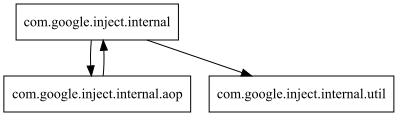
\includegraphics[scale=0.6]{img/packages_example}
    \caption{\textit{graphviz} įrankio sugeneruotas priklausomybių grafikas}
    \label{img:graphviz}
\end{figure}
Gauti matai, priklausomybiu grafikas, bei bendras sistemos paketų medis yra išvedami į išvesties direktoriją nurodyta \textit{output} argumentu.
Matai, paketų medis grąžinami kaip \textit{latex} formato failai, todėl juos galima iškarto įdėti į darbo projektą, nesirūpinant tinkamu formatavimu,
taip padarant sistemų analizę greitesne bei efektyvesne.
